\documentclass[12pt,letterpaper]{article}

\usepackage{multirow}
\usepackage{listings}
\lstset{frame=tb,
language=Matlab,
aboveskip=3mm,
belowskip=3mm,
showstringspaces=false,
columns=flexible,
basicstyle={\small\ttfamily},
numbers=none,
numberstyle=\tiny\color{gray},
keywordstyle=\color{blue},
commentstyle=\color{dkgreen},
stringstyle=\color{mauve},
breaklines=true,
breakatwhitespace=true
tabsize=3
title=\lstname 
}

%                                                                      Package
%********************************************************************************************************************************
\usepackage[margin=1.0in]{geometry}
\usepackage{amsfonts,amsmath,amssymb}
\usepackage[x11names]{xcolor}
\usepackage{colortbl}
\usepackage[pagecolor={green!0!white}]{pagecolor}
\usepackage{tikz}
\usepackage{multirow}
\usepackage{lscape}
\usepackage{float}
\usepackage{dcolumn}
\usepackage{booktabs}
%********************************************************************************************************************************

%                                                                   Code environment
%********************************************************************************************************************************
\usepackage{listings}
\usepackage{color}

\definecolor{dkgreen}{rgb}{0,0.6,0}
\definecolor{gray}{rgb}{0.5,0.5,0.5}
\definecolor{mauve}{rgb}{0.58,0,0.82}

\lstset{frame=tb,language=python,aboveskip=3mm,belowskip=3mm,showstringspaces=false,columns=flexible,basicstyle={\small\ttfamily},
	 numbers=none,numberstyle=\tiny\color{gray},keywordstyle=\color{blue},commentstyle=\color{dkgreen},stringstyle=\color{mauve},
	  breaklines=true,breakatwhitespace=true,tabsize=3}
%********************************************************************************************************************************	  

%                                                                     Newcommand
%********************************************************************************************************************************
\newcommand{\R}{\mathbf{R}}				%Real
\newcommand{\Z}{\mathbf{Z}}				%Integer
\newcommand{\Q}{\mathbf{Q}}				%Rational
\newcommand{\B}{\mathbf{B}}				%Binary

\newcommand{\rank}[1]{\textit{\textbf{rank}}(#1)}		%rank
\newcommand{\dimension}[1]{\textit{\textbf{dim}}(#1)}		%dimension
\newcommand{\conv}[1]{\textit{\textbf{conv}}(#1)}		%Convex hull
\newcommand{\recc}[1]{\textit{\textbf{recc}}(#1)}		%Reccsion cone
\newcommand{\lin}[1]{\textit{\textbf{lin}}(#1)}			%linearity space
\newcommand{\interior}[1]{\textit{\textbf{int}}(#1)}			%interior points set
\newcommand{\bound}[1]{\textit{\textbf{bd}}(#1)}			%bound set
\newcommand{\ri}[1]{\textit{\textbf{ri}}(#1)}			%relative interior points set
\newcommand{\cl}[1]{\textit{\textbf{cl}}(#1)}			%closure
\newcommand{\ie}{\textit{i.e.}}					%i.e.				
\newcommand{\m}[1]{~\mbox{#1}~}					%mbox
\newcommand{\mc}[1]{\mathcal{#1}}				%mathcal
\newcommand{\mbb}[1]{\mathbb{#1}}				%mathbb
\newcommand{\norm}[1]{\|#1\|_2}				%2-norm
\newcommand{\todo}[1]{{\color{red}{#1}}}  %highlight on red

\DeclareMathOperator{\diag}{diag} 

\newcommand{\Qs}[1]{\ \par\noindent{\textsc{\large{Question}}}~\textbf{\large{#1}}.}	%Question style
\newcommand{\sub}[1]{\textbf{(#1)}:}								%subproblem
\newcommand{\co}[1]{\ \par \textbf{(\emph{#1})}}						%cooperator/reference

\newcommand{\rowline}{~\\ \hrule ~\\}								%rowline
%********************************************************************************************************************************

%                                                                   Newenvironment
%********************************************************************************************************************************
\newenvironment{solution}{\par\noindent\textbf{\emph{Solution}:}}{\hfill $\diamondsuit$\par}
\newenvironment{proof}{\par\noindent\textbf{\emph{Proof}:}}{\hfill $\Box$\par}
%********************************************************************************************************************************
 
%                                                                         Title
%********************************************************************************************************************************
\newcommand{\ip}[2]{
\noindent \textsc{Homework \##1}\hfill \textbf{Xi He}~~\today\\
ISE418 -- Integer Programming \hfill \textbf{Due:} #2, 2014\\
\begin{tikzpicture}\draw (1,1) -- (17.5,1);\end{tikzpicture}}      				%Integer Programming Homework

\newcommand{\ipm}[2]{
\noindent \textsc{Midterm \##1}\hfill \textbf{Xi He}~~\today\\
ISE418 -- Integer Programming \hfill \textbf{Due:} #2, 2014, 5:59 PM\\
\begin{tikzpicture}\draw (1,1) -- (17.5,1);\end{tikzpicture}}      				%Integer Programming Midterm

\newcommand{\pat}[2]{
\noindent \textsc{Homework \##1}\hfill \textbf{Xi He}~~\today\\
CSE426 -- Pattern Recognition \hfill \textbf{Due:} #2, 2015\\
\begin{tikzpicture}\draw (1,1) -- (17.5,1);\end{tikzpicture}}					%Intro of Lp Homework

\newcommand{\patfinal}[1]{
\noindent \textsc{Final Project}\hfill \textbf{Xi He}~~\today\\
CSE426 -- Pattern Recognition \hfill \textbf{Due:} #1, 2015\\
\begin{tikzpicture}\draw (1,1) -- (17.5,1);\end{tikzpicture}}   

\newcommand{\lpb}[2]{
\noindent \textsc{Bonus \##1}\hfill \textbf{Xi He}~~\today\\
ISE406 -- Intro of LP \hfill \textbf{Due:} #2, 2014\\
\begin{tikzpicture}\draw (1,1) -- (17.5,1);\end{tikzpicture}}					%Intro of Lp Bonus

\newcommand{\con}[2]{
\noindent \textsc{Homework \##1}\hfill \textbf{Xi He}~~\today\\
ISE417 -- nonlinear programming \hfill \textbf{Due:} #2, 2015\\
\hrule}
%\begin{tikzpicture}\draw (1,1) -- (17.5,1);\end{tikzpicture}}					%Convex Anal. and Opt. 

\pagenumbering{Roman}                                                                              %pagenumber
%********************************************************************************************************************************

\newcommand*{\starnr}{\stepcounter{equation}\tag{\theequation}}
\makeatletter
\newenvironment{Salign}
  {\start@align\@ne\st@rredtrue\m@ne}
  {\starnr\endalign}
\makeatother

\begin{document}
\patfinal{May 1}

\section{Introduction}
In this report, we test four classifiers on given data set II. We have four separate sets: A, B, C and D in data set II, which in total includes $10$ uppercase character classes in a single type 'Times Roman'. Furthermore, we find a new feature and rebuild classifier which has the best performance among those four classifiers. Finally, we design a new classifier by $SVM$ and compare the classified result with other classifier. Note that throughout all this report, we choose set A as training set and then using classifier to classify all sets A, B, C and D.

We use $20$-dimension moments feature for the first four classifiers, and we state the $20$ moment used in the implementation as following.
\begin{equation}
M_{i,j} \quad\m{where} i = 1,2,\dots,6\m{and}j = i,\dots,7-i, \m{exclude} M_{6,1}.
\end{equation}

By using this $20$-dimension moments feature, we training data set A with the following four classifiers
\begin{description}
\item[\todo{M1.}] Moment-space minimum-distance classifier
\item[\todo{M2.}] Moment-space classifier with identical covariances
\item[\todo{M3.}] 1NN in moment space
\item[\todo{M4.}] 5NN in moment space (breaking ties lexically).
\end{description}

After this, we choose new feature as the mean of pixel space in each position, i.e., in $256$-dimension space. By making use of this feature on those four classifiers, we notice that the best performance comes from classifier $M3$ with $256$-dimension pixel space, so we called this classifier as
\begin{description}
\item[\todo{M5.}] 1NN in pixed space.
\end{description}

Finally, we explore $SVM$ classifier which based on the two-labels classifier function $svmtrain$ and $svmclassify$. Actually, what we did to use this method is test each two classes separately (which is $45$ times compare for each sample), and then choose the most frequent correct answer to be the classified result. We also train and test this classifier in pixel space. We call this classifier as 
\begin{description}
\item[\todo{M6.}] SVM in pixed space.
\end{description}

In section \ref{sec: summary_error_table}, we summary error table for each method when train on set A and test on set A, B, C and D respectively.

\section{Summary Error Table}\label{sec: summary_error_table}
\begin{table}[H]
\centering
\begin{tabular}{c || c c c c}
	Classifier  &  A & B & C & D \\
	\hline
            M1 & 201 & 209 & 231 & 196\\
            M2 &  39& 39 &  49& 37\\
            M3 &  0&  92& 114 & 105\\
           M4 &  128& 143 & 158 & 164\\
           \hline
        M5 &  0& 13 & 16 & 17\\
    	M6 &  0& 8 & 9 & 4\\
\end{tabular}	
 \caption{Error table for M1-M6 on data set II}
\end{table}

We learn that in moment space, M2 shows the best classification result. Then, by definition, we derive the best average error rate is
\begin{equation}
 E = \frac{39+49+37}{3} \approx 42.
\end{equation} 

One can see that both $M5$ and $M6$ cut $E$ by at least a factor of two, which means these two methods satisfies requirement of this report.

\section{Confusion Tables}\label{sec: Confusion_tables}

In this section, we list all six confusion table of these six classifiers. Note that the confusion table is derived as training on set A and testing on entire data set II. In other word, each of the confusion table is the sum of four confusion table by using a classifier on training on set A and testing on A, B, C and D respectively.
\begin{figure}[H]
\centering
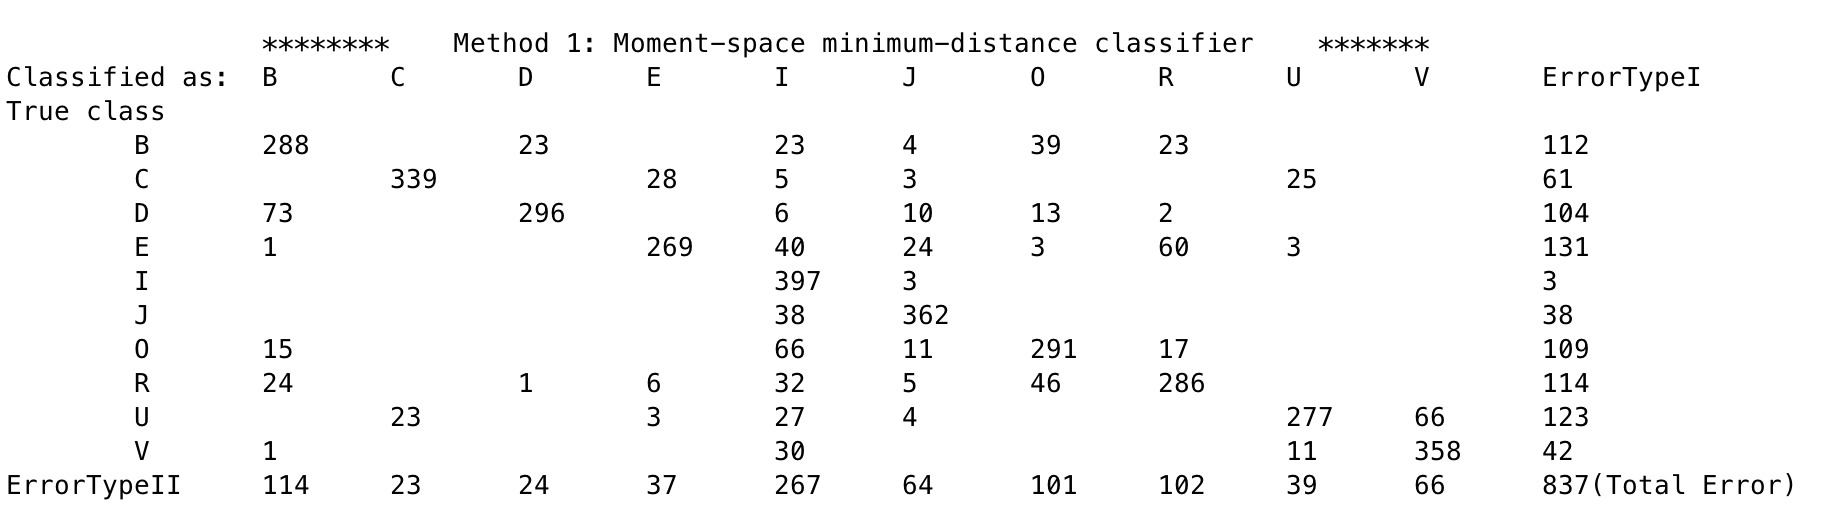
\includegraphics[width=0.95\textwidth]{1}
\caption{Moment-space minimum-distance classifier}
\end{figure}

\begin{figure}[H]
\centering
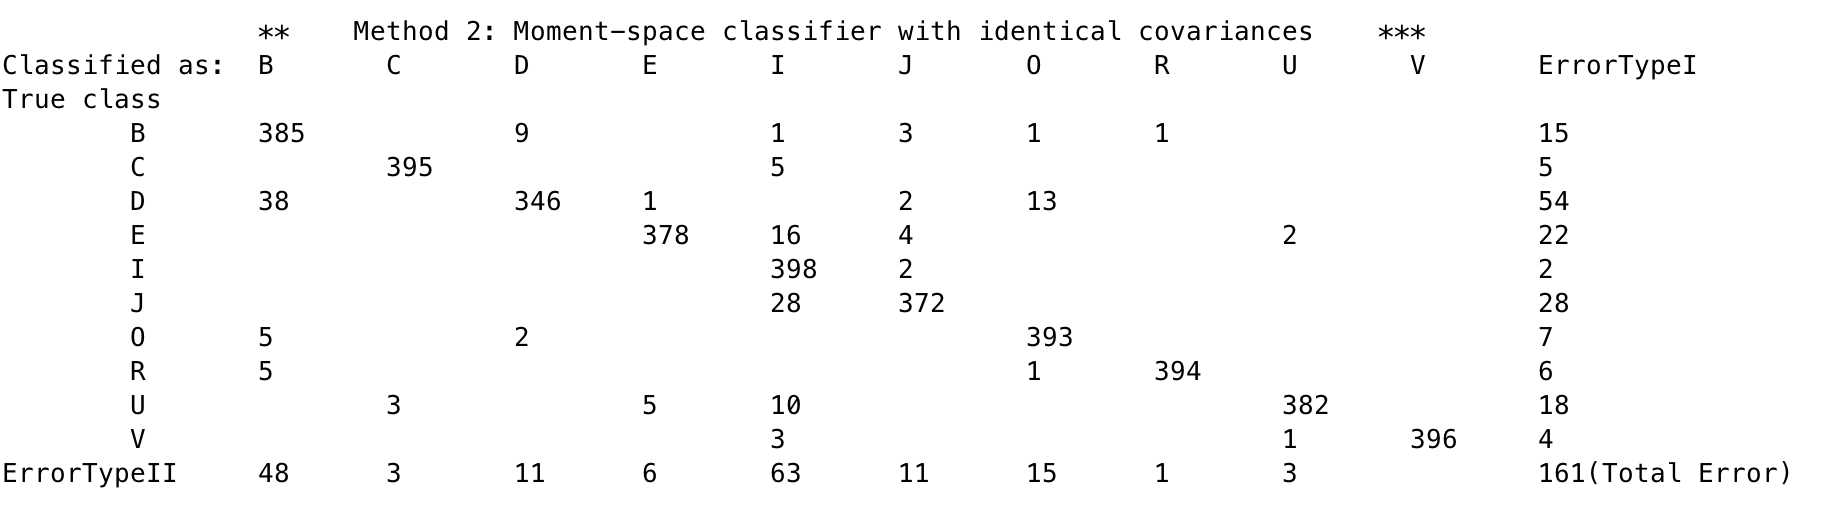
\includegraphics[width=0.95\textwidth]{2}
\caption{Moment-space classifier with identical covariances}
\end{figure}

\begin{figure}[H]
\centering
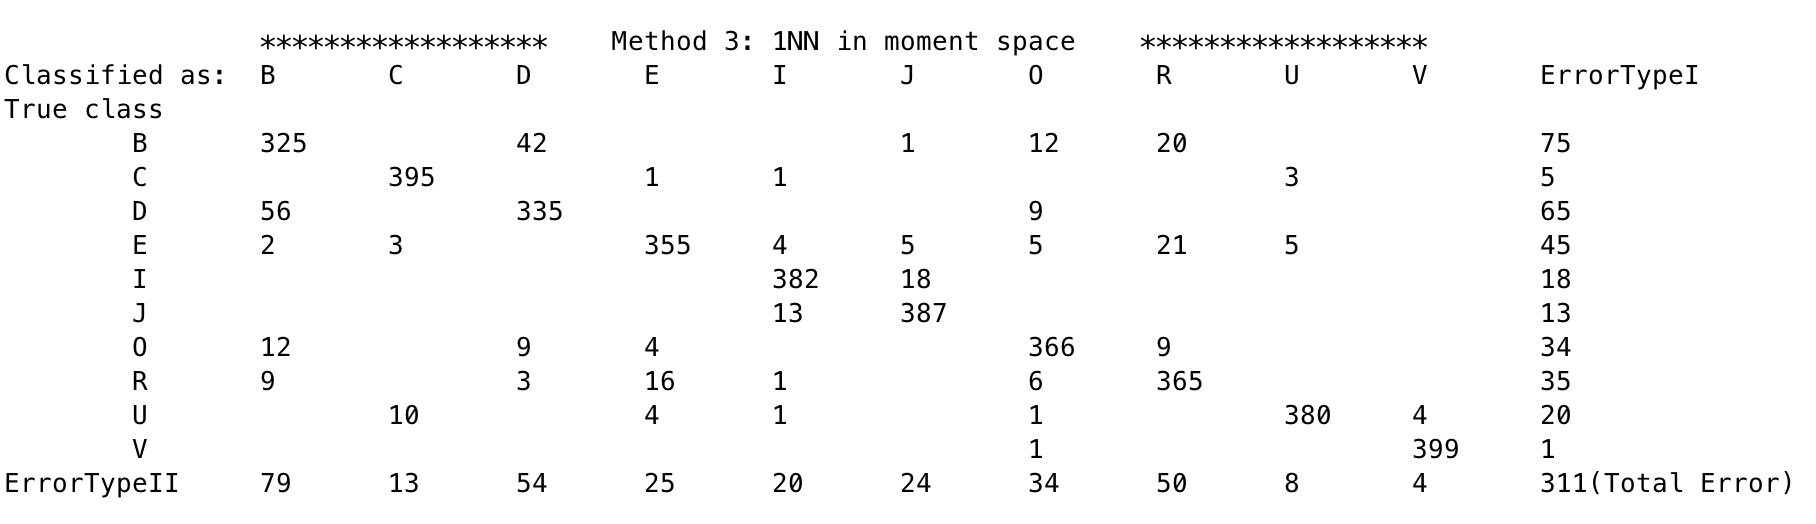
\includegraphics[width=0.95\textwidth]{3}
\caption{1NN in moment space}
\end{figure}

\begin{figure}[H]
\centering
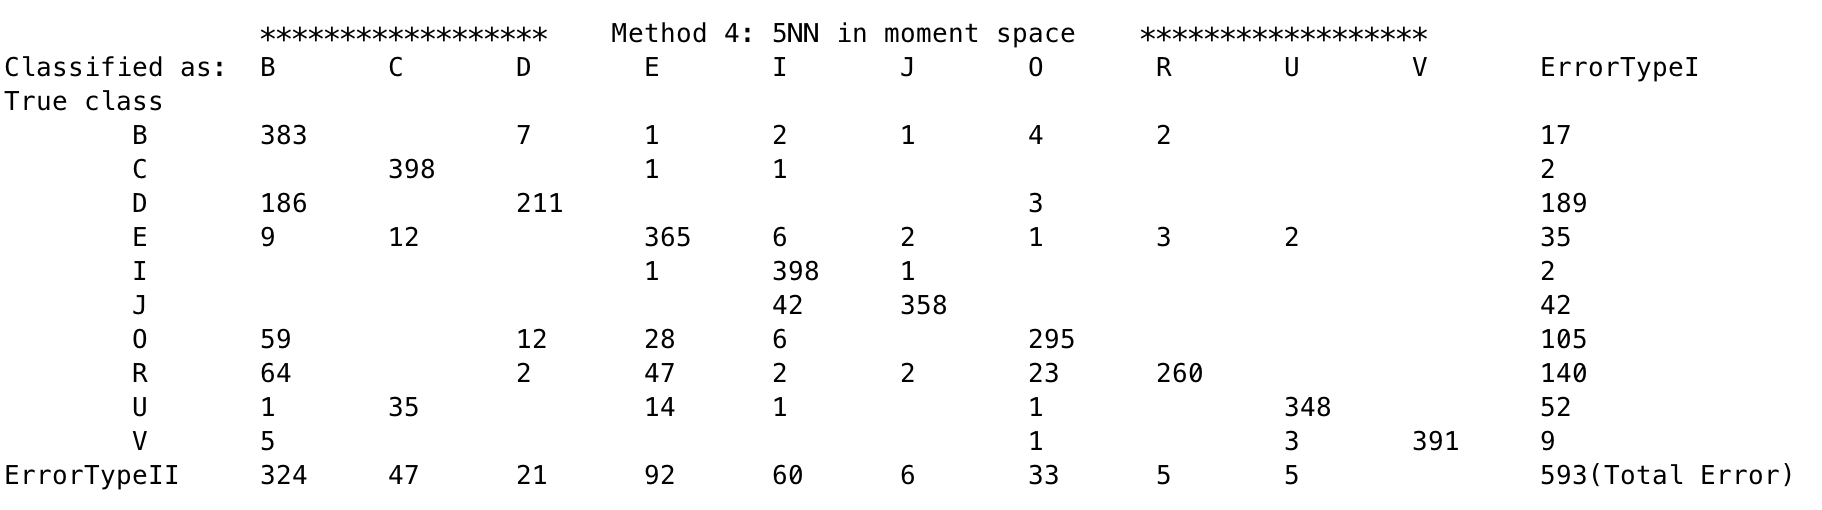
\includegraphics[width=0.95\textwidth]{4}
\caption{5NN in moment space (breaking ties lexically)}
\end{figure}

\begin{figure}[H]
\centering
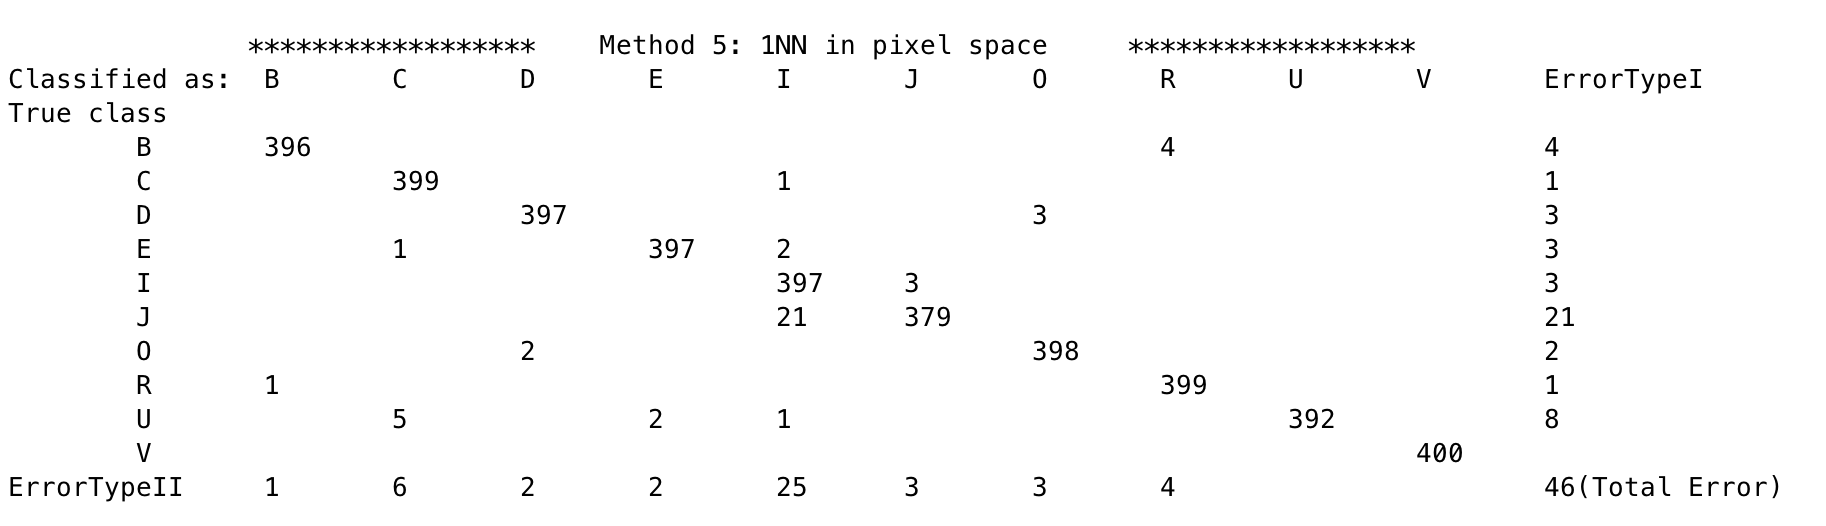
\includegraphics[width=0.95\textwidth]{5}
\caption{1NN in pixed space}
\end{figure}

\begin{figure}[H]
\centering
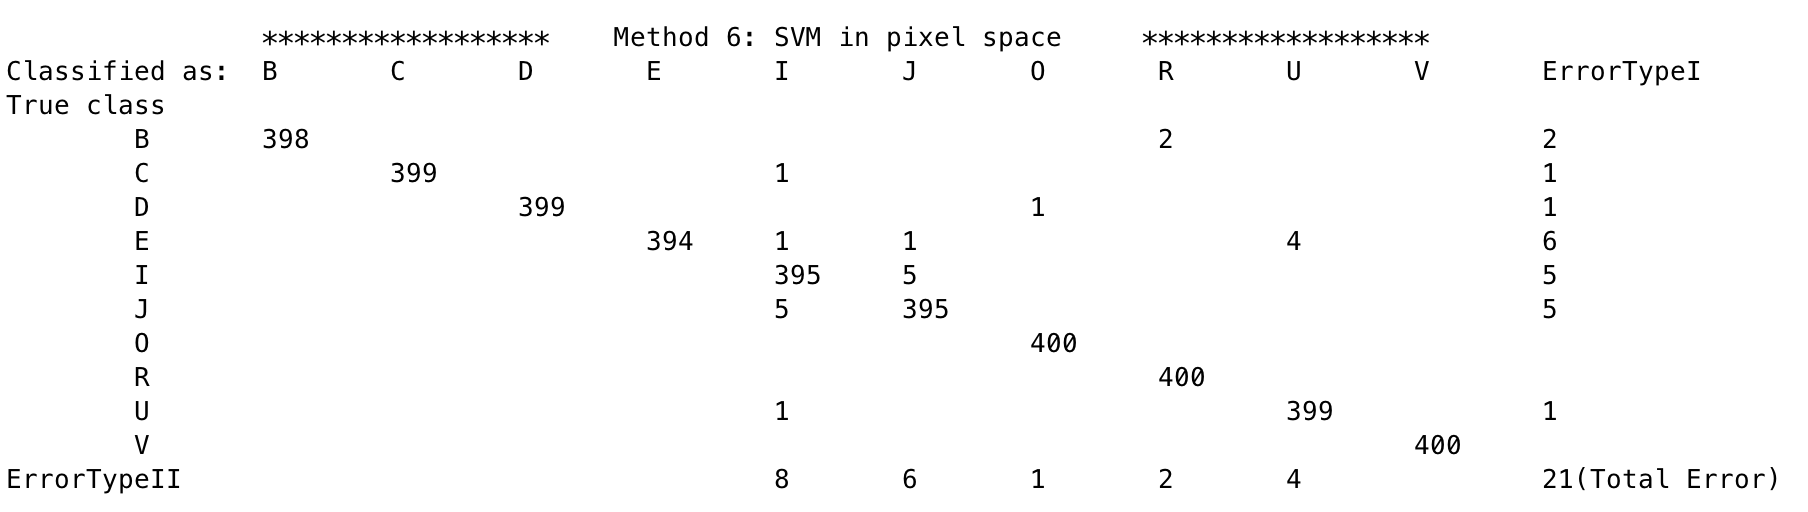
\includegraphics[width=0.95\textwidth]{6}
\caption{SVM in pixed space}
\end{figure}

\section{Discussion}

From error table in section \ref{sec: summary_error_table} and confusion table in section \ref{sec: Confusion_tables}, we can say that it's better to apply pixel feature and svm method to attain a relative low error rate. However, we have the following execution time for each classifier.

\begin{table}[H]
\centering
\begin{tabular}{c || c c c c c c}
    Classifier  &  M1 & M2 & M3 & M4 &M5 &M6 \\
    \hline
    CPUtime(s) & 0.1718 & 0.7498 & 9.4580 & 9.4787 & 11.9983 & 84.2689
\end{tabular}   
\caption{Time cost for M1-M6 on data set II}
\end{table}

From table 2, we may see that M5 and M6, who have relatively high classification accuracy, need more computation to obtain the result. And roughly speaking, nearest neighborhood methods are more costly since it need do more comparison and multiplication. With respect to M6, which is based on SVM method, it costly much more time. However, it is reasonable since to derive the classified result, we should run 45 times classification process, which is costly.

\section{Program Listings}

This section includes all the implementation details for this project. All the results can be computed by these program.

\lstinputlisting[language=Matlab, caption=\lstname]{RESULT.m}

\lstinputlisting[language=Matlab, caption=\lstname]{Input_data.m}
\lstinputlisting[language=Matlab, caption=\lstname]{deal_data_moment.m}
\lstinputlisting[language=Matlab, caption=\lstname]{classify_first.m}
%\lstinputlisting[language=Matlab, caption=\lstname]{classify_first_improved.m}
\lstinputlisting[language=Matlab, caption=\lstname]{classify_second.m}
\lstinputlisting[language=Matlab, caption=\lstname]{classify_third.m}
\lstinputlisting[language=Matlab, caption=\lstname]{classify_fourth.m}
%\lstinputlisting[language=Matlab, caption=\lstname]{classify_fifth.m}
\lstinputlisting[language=Matlab, caption=\lstname]{deal_data_pixel.m}
%stinputlisting[language=Matlab, caption=\lstname]{classify_first_pixel.m}
%\lstinputlisting[language=Matlab, caption=\lstname]{classify_first_improved.m}
%\lstinputlisting[language=Matlab, caption=\lstname]{classify_second_pixel.m}
%\lstinputlisting[language=Matlab, caption=\lstname]{classify_third_pixel.m}
%\lstinputlisting[language=Matlab, caption=\lstname]{classify_fourth_pixel.m}
\lstinputlisting[language=Matlab, caption=\lstname]{classify_fifth_pixel.m}
\lstinputlisting[language=Matlab, caption=\lstname]{classify_sixth_pixel.m}

\newpage
\lstinputlisting[language=Matlab, caption=\lstname]{cen_mon.m}
\lstinputlisting[language=Matlab, caption=\lstname]{discrim.m}
\lstinputlisting[language=Matlab, caption=\lstname]{print.m}
\end{document} 